
\chapter{Implementation details}\label{chap:implementation-details}

\section{Scala Commander}

Scala Commander is a simple desktop application built as a proof-of-concept of the library \emph{Scala.React}, \emph{Scala-Swing}, and of Scala as a language of choice for general application development. It is built using the Model-View-Controller design pattern (see section \ref{sec:model-view-controller}), where the model consists of Scala.React \emph{event streams} and \emph{signals}, the view consists of Scala-Swing components, and the operations in the controller are implemented using Scala.React \emph{reactors}.

Scala Commander a simple \emph{orthodox file manager} application, consisting of two panels showing the contents of one directory each (see figure \ref{fig:scomm_main}). The user can navigate to an arbitrary directory, can select files and folders, and can execute operations on the selection such as copying, moving, or deletion.



\begin{figure}[h!] 
  \centering
    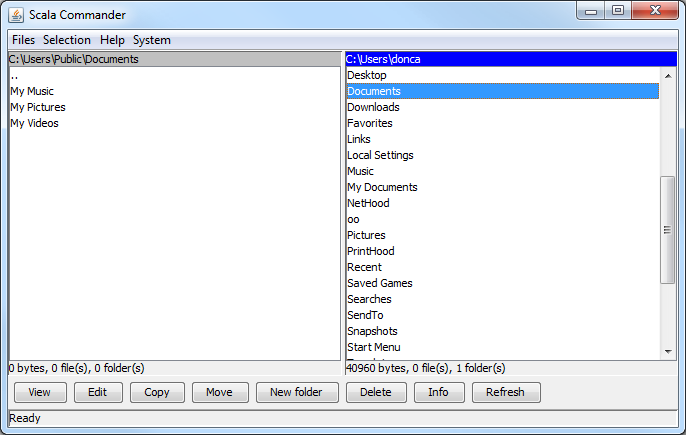
\includegraphics[width=1\textwidth]{images/scala-commander-main.png}
  \caption{Scala-Commander.}
  \label{fig:scomm_main}  
\end{figure}

\subsection{The directory list}

The directory list model is built on Scala.React signals (variables and functions), event sources and reactors.

The model contains entries in the form of the path and the displayed name:
\begin{lstlisting}
case class FileEntry(path: Path, name: String)
\end{lstlisting}

The model's state consists of three signal \emph{variables} and two (derived) signal \emph{functions}:
\begin{itemize}
\item \texttt{currentDirectory} --- the current directory (as a \texttt{java.nio.Path} object);
\item \texttt{selectedPaths} --- the set of selected paths;
\item \texttt{active: Var[Boolean]} --- a flag showing whether the directory list is considered active or inactive;
\item \texttt{currentDirContents} --- holds, as a list of files, the contents of the current directory based on the variable  \texttt{currentDirectory};
\item \texttt{selectionInfo} --- holds an aggregated info of what the user selected, based on \texttt{selectedPaths} and \texttt{currentDirectory}.
\end{itemize}

The model also contains three event sources, each representing an \emph{action} that is defined on the directory list:
\begin{itemize}
\item \texttt{goToParent: EventSource[Unit]} --- go to the parent of the current directory (if it exists);
\item \texttt{goToIndex: EventSource[Int]} --- go to the directory identified by the given index (index of the list \texttt{currentDirContents});
\item \texttt{selectIndices: EventSource[Set[Int]]} --- select paths identified by the given set of indexes.
\end{itemize}

Finally, the model consists of four reactors that glue together the model's state and the event sources: whenever a certain event source emits, they alter the model's state accordingly. The four reactors are the following:
\begin{itemize}
\item \texttt{goToParentReactor} --- awaits the next \texttt{goToParent} event in a loop, after which it sets the variable \texttt{currentDirectory} to the parent of the current directory (if it exists);
\item \texttt{goToIndexReactor} --- awaits the next index of \texttt{goToIndex} in a loop, after which it sets current directory to the directory identified by the given index based on the current value of \texttt{currentDirContents};
\item \texttt{selectIndicesReactor} --- awaits the next index set of \texttt{selectIndices} in a loop, after which it sets the variable \texttt{selectedPaths} based on the current value of \texttt{currentDirContents};
\item \texttt{activeReactor} --- awaits the next value of the signal \texttt{active}, and if it is set to false, clears the selection (sets the variable \texttt{selectedPaths} to the empty set).
\end{itemize}

Because of Scala.React's automatic 

\begin{figure}[h!]
\centering
\begin{tikzpicture} 
\umlemptyclass[x=0, y=-2]{DiskState}
\umlemptyclass[x=3, y=0]{DirectoryListModel}
\umlemptyclass[x=9, y=0]{DirectoryListController} 
\umlemptyclass[x=6, y=-2]{DirectoryListView} 
\umluniassoc[geometry=--]{DirectoryListModel}{DiskState} 
\umluniassoc[geometry=--]{DirectoryListController}{DirectoryListModel} 
\umluniassoc[geometry=--]{DirectoryListController}{DirectoryListView} 
\umluniassoc[geometry=--]{DirectoryListView}{DirectoryListModel} 
\umlVHdep{DirectoryListModel}{DirectoryListView}
\umlHVdep{DirectoryListView}{DirectoryListController}
\umlVHdep{DiskState}{DirectoryListModel}
\end{tikzpicture}
\caption{The directory list components.}
\label{fig:mvc_pattern}
\end{figure}



\section{Test auditing}\label{sec:test-auditing}

\subsection {Non-independent tests}

Test suites testing even relatively complex applications can easily contain some hundred tests. Because UI tests, by their nature, typically take much time, the total run time of an entire test suite is usually important. In order to keep the overall runtime at minimum, it is typical to avoid the creation, initialization and the destruction of the individual UI components for each test (which might also be difficult or impossible depending on the architecture of the application). A possible option is to test entire applications and to reuse the same components between the tests.

The problem with testing entire applications throughout entire test suites is that the tests can become dependent on the internal state of the application and on the state of the UI. Thus, it is possible for one test to affect the outcome of another, e.g. one failing test can leave the application in such a state that no other further tests will pass. Having non-independent tests can lead to very fragile and unstable test systems and thus should be avoided as much as possible.

Unstable test system can very difficult to cope with. Tests can seemingly fail randomly, and it can be very difficult to reproduce failures that originate from typically a subtle change in the application's state that was made by a previous test (possibly executed multiple tests before). FEST supports saving screenshots anytime during a test, but the test must explicitly save it and it is usually done only on errors. Since in the case of unstable tests, the errors typically manifest themselves only in the tests that are affected by the erroneous tests' side effects, saving screenshots for failing tests does not help much on its own.

Understanding the data flow of all the tests of an entire test suite, knowing all the operations that were made on the application's state, along with screenshots made after all important steps can greatly reduce the debugging efforts of an unstable test suite and can benefit the test development and maintenance process.

\subsection {AspectJ-based auditing}

A possible implementation of the auditing is by using AspectJ. The runtime system could rely on using join points defined by automatically generated pointcuts, and by using advices wrapping around the join points, the entire method invocation context (stack trace, method arguments) can be stored (logged). \cite{AOPwiki} From the context of each method invocation, an execution tree can then be built and visualized.

The pointcuts could be generated for the methods of the classed in the test, user action, adapter, fixture, driver or robot layers. The deeper auditing goes through the layers, the more runtime data is gathered and the bigger is the performance cost of the auditing. Thus, it is important to make the set of the audited layers and methods configurable.

Screenshots could be similarly generated after each user action (or adapter operation) of a test.

\subsection {Formatting the audited data}

Since the runtime data set can be very huge for long tests runs, it is important to provide views that presents the data in an easily accessible, intuitive and adaptive form. 

A possible implementation is to generate an HTML page that contains all the data in the form of a pivot table, with a tree axis showing the call hierarchy, and the columns presenting the method arguments and other context info. The pivot table would support drill-down in the call hierarchy. This table would support the following:
\begin{itemize}
\item Closing and expanding nodes (method calls) in the call hierarchy;
\item Filtering and sorting by the context data (e.g. method names, arguments, annotations).
\end{itemize}

The following is a simple example of a test of a text editor application consisting of the following steps:
\begin{itemize}
\item create a new text file
\item enter the text ``hello'' and `` world'', respectively
\item save the text file to the disk
\item assert that the editor shows the file name in the window's title
\item assert that the file exists on the disk and has the appropriate content
\end{itemize}

Table \ref{fig:formatted_audited_data_report} shows the method calls only of the test, user action and adapter layers, along with the arguments and the return values (if applicable).

\begin{table}
\caption{Formatted audited data report}
%\rowcolors{2}{gray!25}{white}
\begin{tabular}{l l c}
%\rowcolor{gray!50}
\hline\hline

Method call & Arguments & Returns \\ [0.5ex] % inserts table heading
\hline 

\hskip 0cm EditorTest.saveNewTextFile & & PASSED \\
\hskip 3mm   EditorUserActions.createNewTextFile & & \\
\hskip 6mm     MenuAdapter.clickFileMenu & & \\ 
\hskip 6mm     MenuAdapter.clickNewTextFileMenuItem & & \\ 
\hskip 3mm   EditorUserActions.enterText & text=''hello'' & \\
\hskip 6mm     TextAreaAdapter.getCaretPosition & & 0 \\
\hskip 6mm     TextAreaAdapter.insertText & position=0, text=''hello'' & \\
\hskip 3mm   EditorUserActions.enterText & text=''world'' & \\
\hskip 6mm     TextAreaAdapter.getCaretPosition & & 5 \\
\hskip 6mm     TextAreaAdapter.insertText & position=5, text='' world'' & \\
\hskip 3mm   EditorUserActions.saveCurrentEditor & filename=''C:{\textbackslash}helloWorld.txt'' & \\
\hskip 6mm     MenuAdapter.clickFileMenu & & \\
\hskip 6mm     MenuAdapter.clickSaveMenuItem & & \\
\hskip 6mm     DialogAdapter.setFileName & filename=''C:{\textbackslash}helloWorld.txt'' & \\
\hskip 6mm     DialogAdapter.clickSaveButton & & \\
\hskip 6mm     DialogAdapter.expectToDisappear & & \\	 
\hskip 3mm   EditorUserActions.expectTitle & title=''helloWorld'' & \\
\hskip 6mm     MainWindowAdapter.expectTitle & title=''My Notepad - helloWorld'' & \\
\hskip 6mm     FileUtils.expectFileContents &
    \begin{tabular}[x]{@{}c@{}}
       path=''C:{\textbackslash}helloWorld.txt", \\
      contents=''hello world''
    \end{tabular} & \\

\hline

\end{tabular}
\label{fig:formatted_audited_data_report}
\end{table}

\section{Automatic EDT dispatch}\label{sec:edt-dispatch}

\subsection{Cumbersome synchronization with EDT}\label{sec:edt-sync}

Since the threading model of Swing recommends that all Swing-component-related operations are to be made on the Swing EDT thread, including those of the tests, it is the test developer's responsibility to delegate all such work to the EDT thread by using FEST-Swing's GuiActionRunner. For tests using the User Action and Adapter design pattern, this can lead to much boilerplate code in the adapter layer. 

A solution to having to manually delegate work to EDT would be to mark the methods that needs to run on EDT with a certain annotation and let the runtime system do the delegation automatically. This would lead to lesser effort from the developer's side, and at the same time, would lead to increased security on the tests' correctness.

There can also be methods that must not be invoked on EDT (e.g. most FEST methods, because they check the contents of event queues). Executing those methods on EDT can lead either to exceptions, to the tests hanging, or simply to incorrect behavior. Marking such methods with a certain annotation and letting the runtime system ensure that the test fails whenever the test executes such a method on EDT would also lead to increased security on the tests' correctness.

\subsection {Automatic EDT dispatch}\label{sec:edt-dispatch}

The operations need to be marked with certain annotations and the runtime system behind the scenes automatically handles the delegation.

\section {Simulated drag-and-drop}\label{sec:simulated-dnd}

\subsection{Defective DnD with Cacio-tta}\label{sec:defective-dnd}

FEST-Swing completely supports mouse gesture-based drag-and-drop (DnD) between Swing components, allowing the tests to cover that part of the application's functionality. However, some limitations (see above \fullref{sec:fest-swing-limitations}) often required the tests system to use the alternative graphics stack implementation named Cacio-tta \cite{Cacio_Tta_FEST} with the known limitation that it does not provide the required system-level support for drag and drop. Thus, in such test systems the mouse gesture-based approach of FEST-Swing's does not work.

A solution would be to programmatically trigger the data export and import operations on the Swing components, thus simulating the drag and drop without any mouse movement. However, because of the platform-dependent nature of the Swing (and AWT) DnD subsystem \cite{IntroDnD} \cite{DnDSubsystem}, this is not trivial to be realized.

\subsection{Drag and drop in Swing - Behind the scenes}\label{sec:dnd-swing}

Let us say that the user, who is running a Java application, wants to drag some text from a list and deposit it into a text field. Briefly, the drag and drop process consists of the following steps \cite{IntroDnD}:

\begin{enumerate}
\item The user has selected a row of text in the source component: the list. While holding the mouse button the user begins to drag the text - this initiates the drag gesture.
\item \label{item:drag-begin} When the drag begins, the list component packages up the data for export and declares what source actions it supports (i.e. COPY, MOVE, or LINK).
\item As the user drags the data, Swing continuously calculates the location and handles the rendering.
\item If the user simultaneously holds the Shift and/or Control key during the drag, this user action is also part of the drag gesture. Typically, an ordinary drag requests the MOVE action. Holding the Control key while dragging requests the COPY action, and holding both Shift and Control requests the LINK action.
\item \label{item:insert-location} Once the user drags the text over the bounds of a text field component, the target is continually polled to see if it will accept or reject the potential drop. As he drags, the target provides feedback by showing the insert location, perhaps an insertion cursor or a high-lighted selection. In the current example, the text field (the current target) allows both re-placement of selected text and insertion of new text.
\item \label{item:import-data} When the user releases the mouse button, the text component imports the data by inspecting the declared source actions and any user action and then it chooses what it wants out of the available options. In the current example, the text field chooses to insert the new text at the point of the drop.
\end{enumerate}

While this might seem like a daunting process, Swing handles most of the work out of the box. The Swing framework is designed so that the developer plug in the details specific to the components, and the rest is automatic.

\subsection {Simulated drag-and-drop}\label{sec:simulated-dnd}

By doing the following steps, the tests can programmatically trigger drag-and-drop:
\begin{enumerate}
\item Trigger an export on the source component (see point \ref{item:drag-begin} above).
\item Set the proper insert location at the destination component (see point \ref{item:insert-location} above).
\item Trigger the import of the data (see point \ref{item:import-data} above).
\end{enumerate}











